%Root main.tex
%---------------------------------------------------------------------------
%第2章　aaa
%---------------------------------------------------------------------------

\chapter{制御理論}
\label{chap:MotorDriveSystem}

\section{系統連系システム}
図(\ref{Fig2.1})に連系リアクトルなし三相系統連系システムの主回路図を示す．本システムは，T-NPC型三相系統連系インバータである．

\begin{figure}[ht]
    \center
    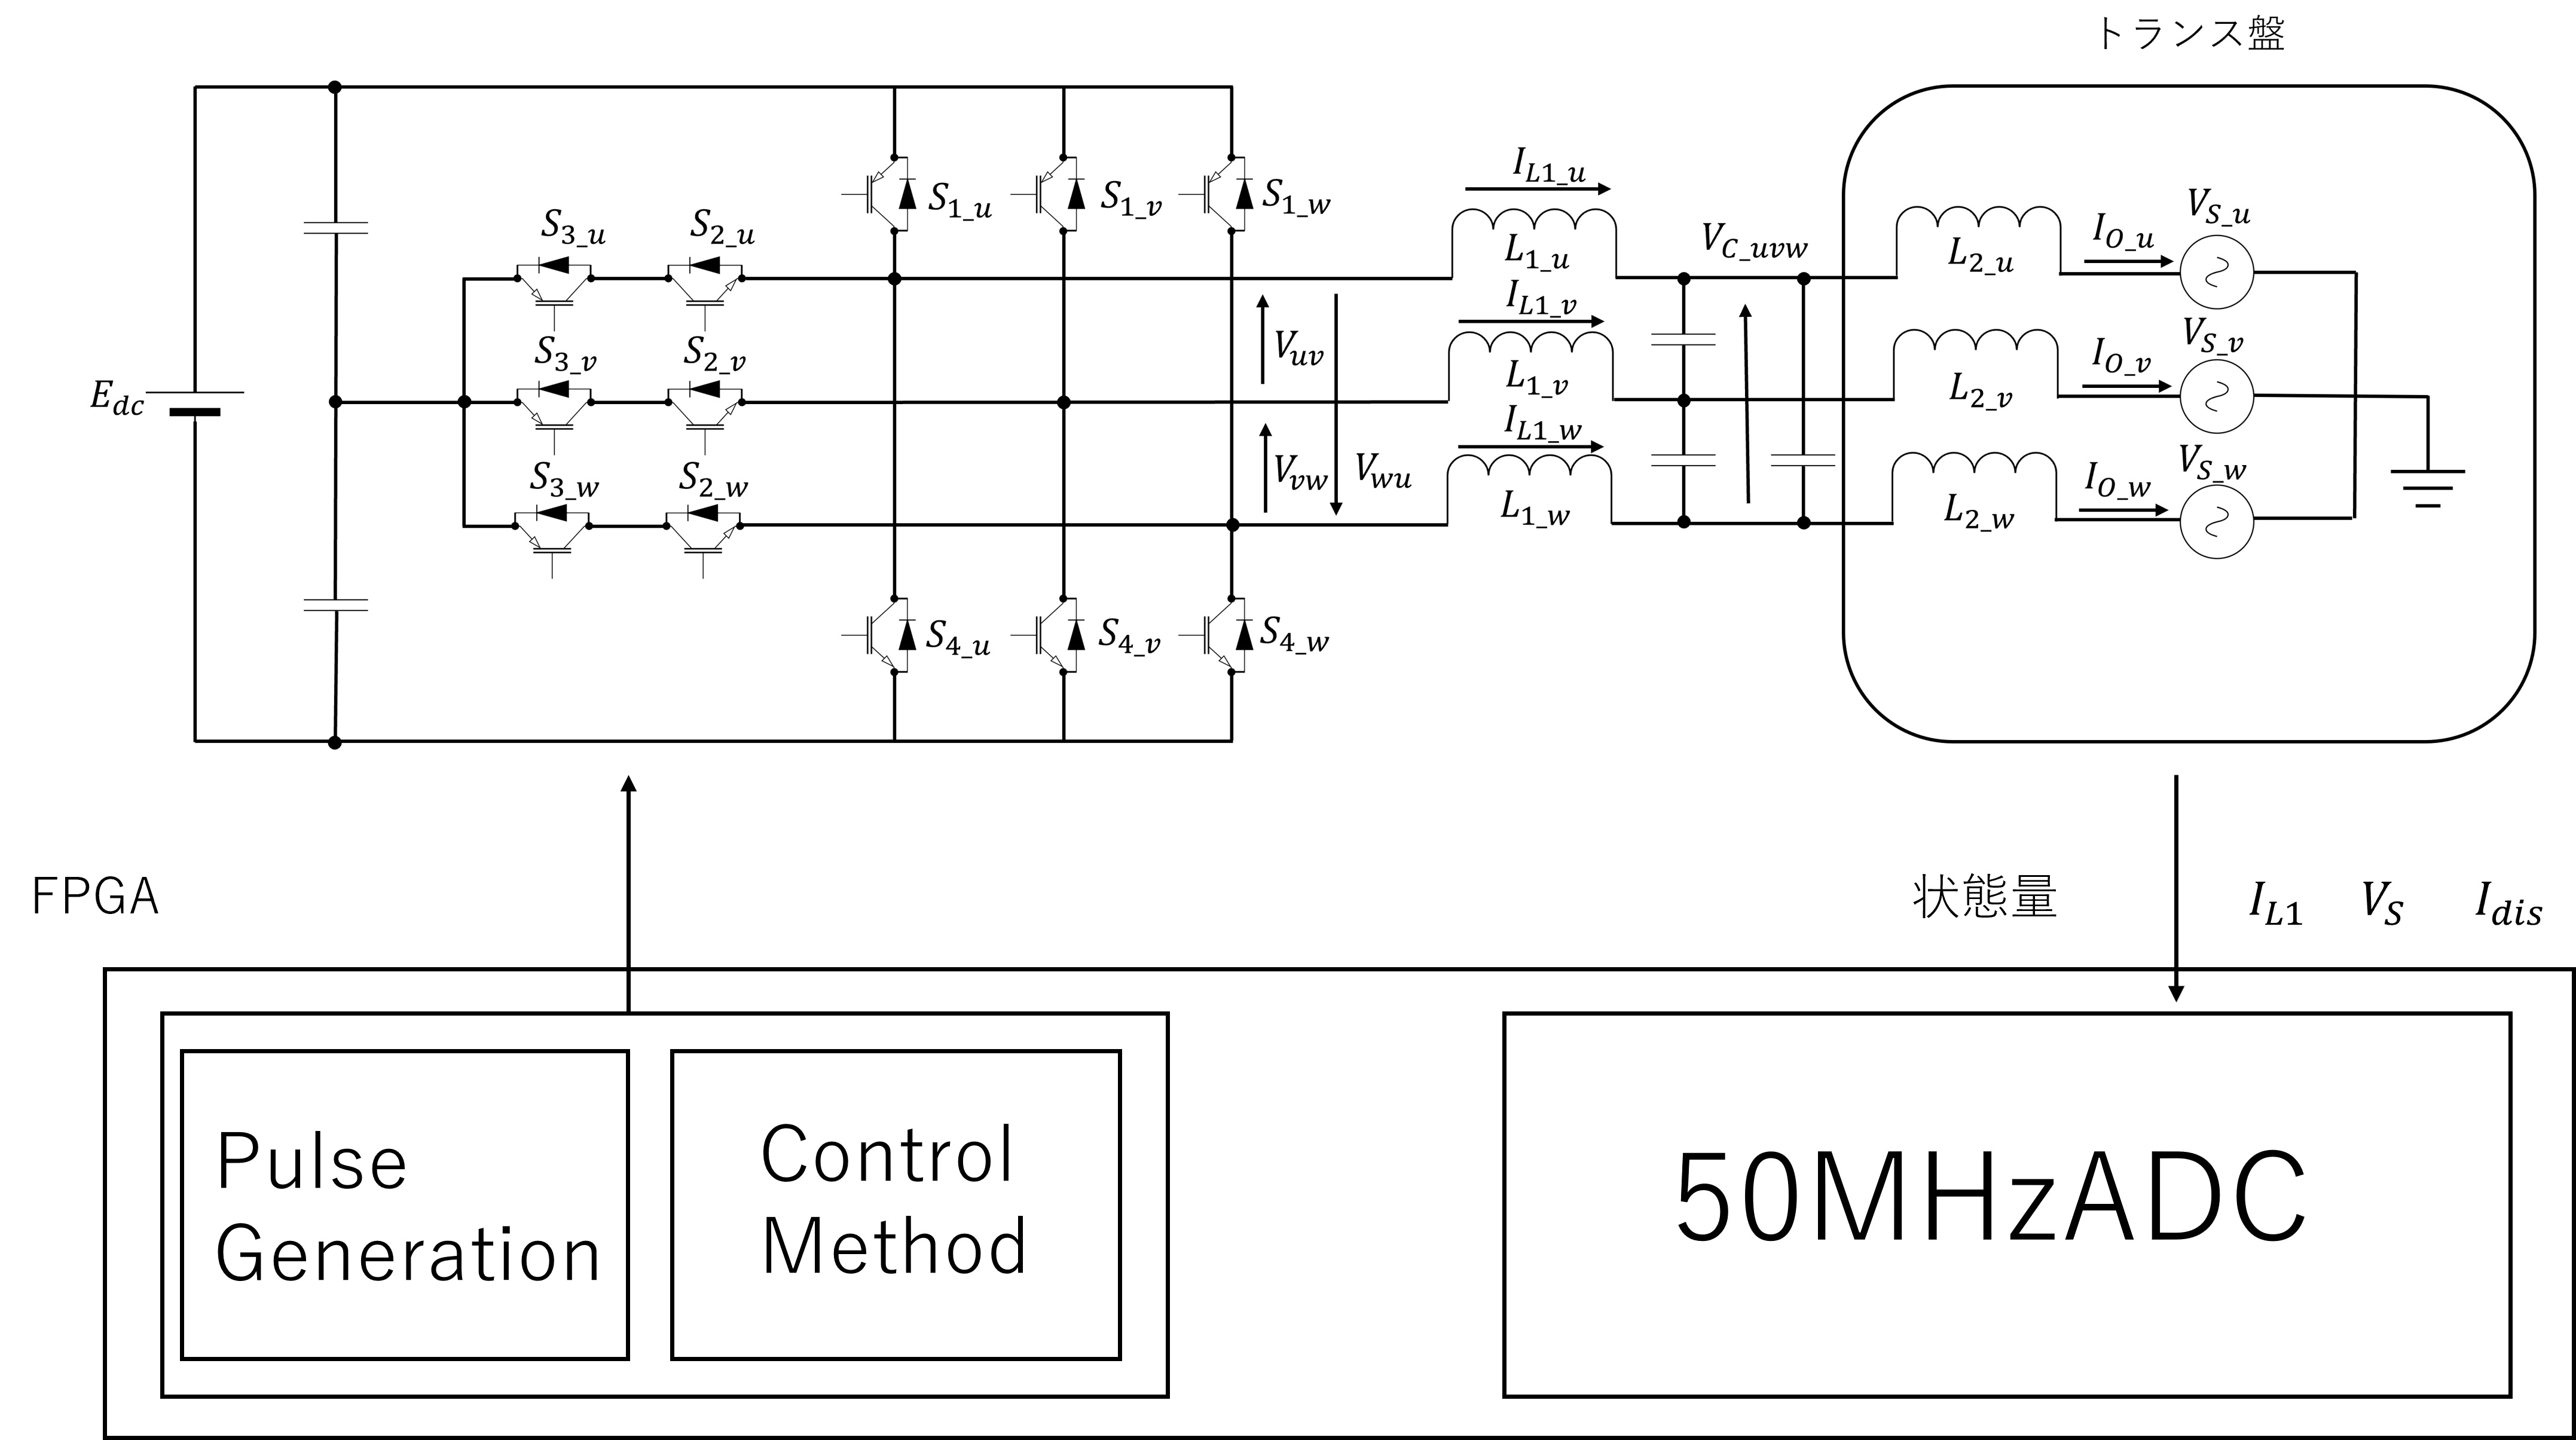
\includegraphics[width=140mm]{image/chapter2/fig.1.png}
    \caption{連系リアクトルなし三相系統連系システムの主回路図}
    \label{Fig2.1}
\end{figure}

%本システムは，分散型電源$E_{dc}$から供給される直流電圧をT-NPC型三相系統連系インバータで$0\si{V}$，\\$\pm $ $E_{dc}\si{V}$の矩形波電圧へ変換する．次にインダクタ$L_{1}$，コンデンサ$C$から構成される$LC$フィルタによって平滑化を行い，交流電圧(インバータ出力電圧)に変換し，連系リアクトル$L_{2}$を介して系統に接続する．また，インバータから連系リアクトル$L_{2}$を通して系統に流れる出力電流$I_{o}$はインバータ出力電圧$V_{c}$と系統電圧$V_{s}$間の電位差及び連系リアクトル$L_{2}$の容量に依存して流れる．

先行研究においては，連系リアクトル$L_{2}$に流れる出力電流$I_{o}$を制御対象としていたが，本研究では，連系リアクトルを制御対象に含まないため，フィルタインダクタ$L_{1}$に流れる電流$IL_{1}$を制御対象とする．

\section{三相二相変換・二相三相変換}
図\ref{Fig2.2}に三相交流のベクトルと二相交流のベクトルの関係図を示す．
本研究では，三相系統連系システムを制御対象として制御を行う．三相のシステムは，単相のシステムと異なり，各相の和が0となる三相平衡の性質から各相を独立して制御することが困難である．そのため，三相二相変換及び，二相三相変換を利用することで三相システムを2つの独立した単相システムとして制御することができる．

\begin{figure}[ht]
    \center
    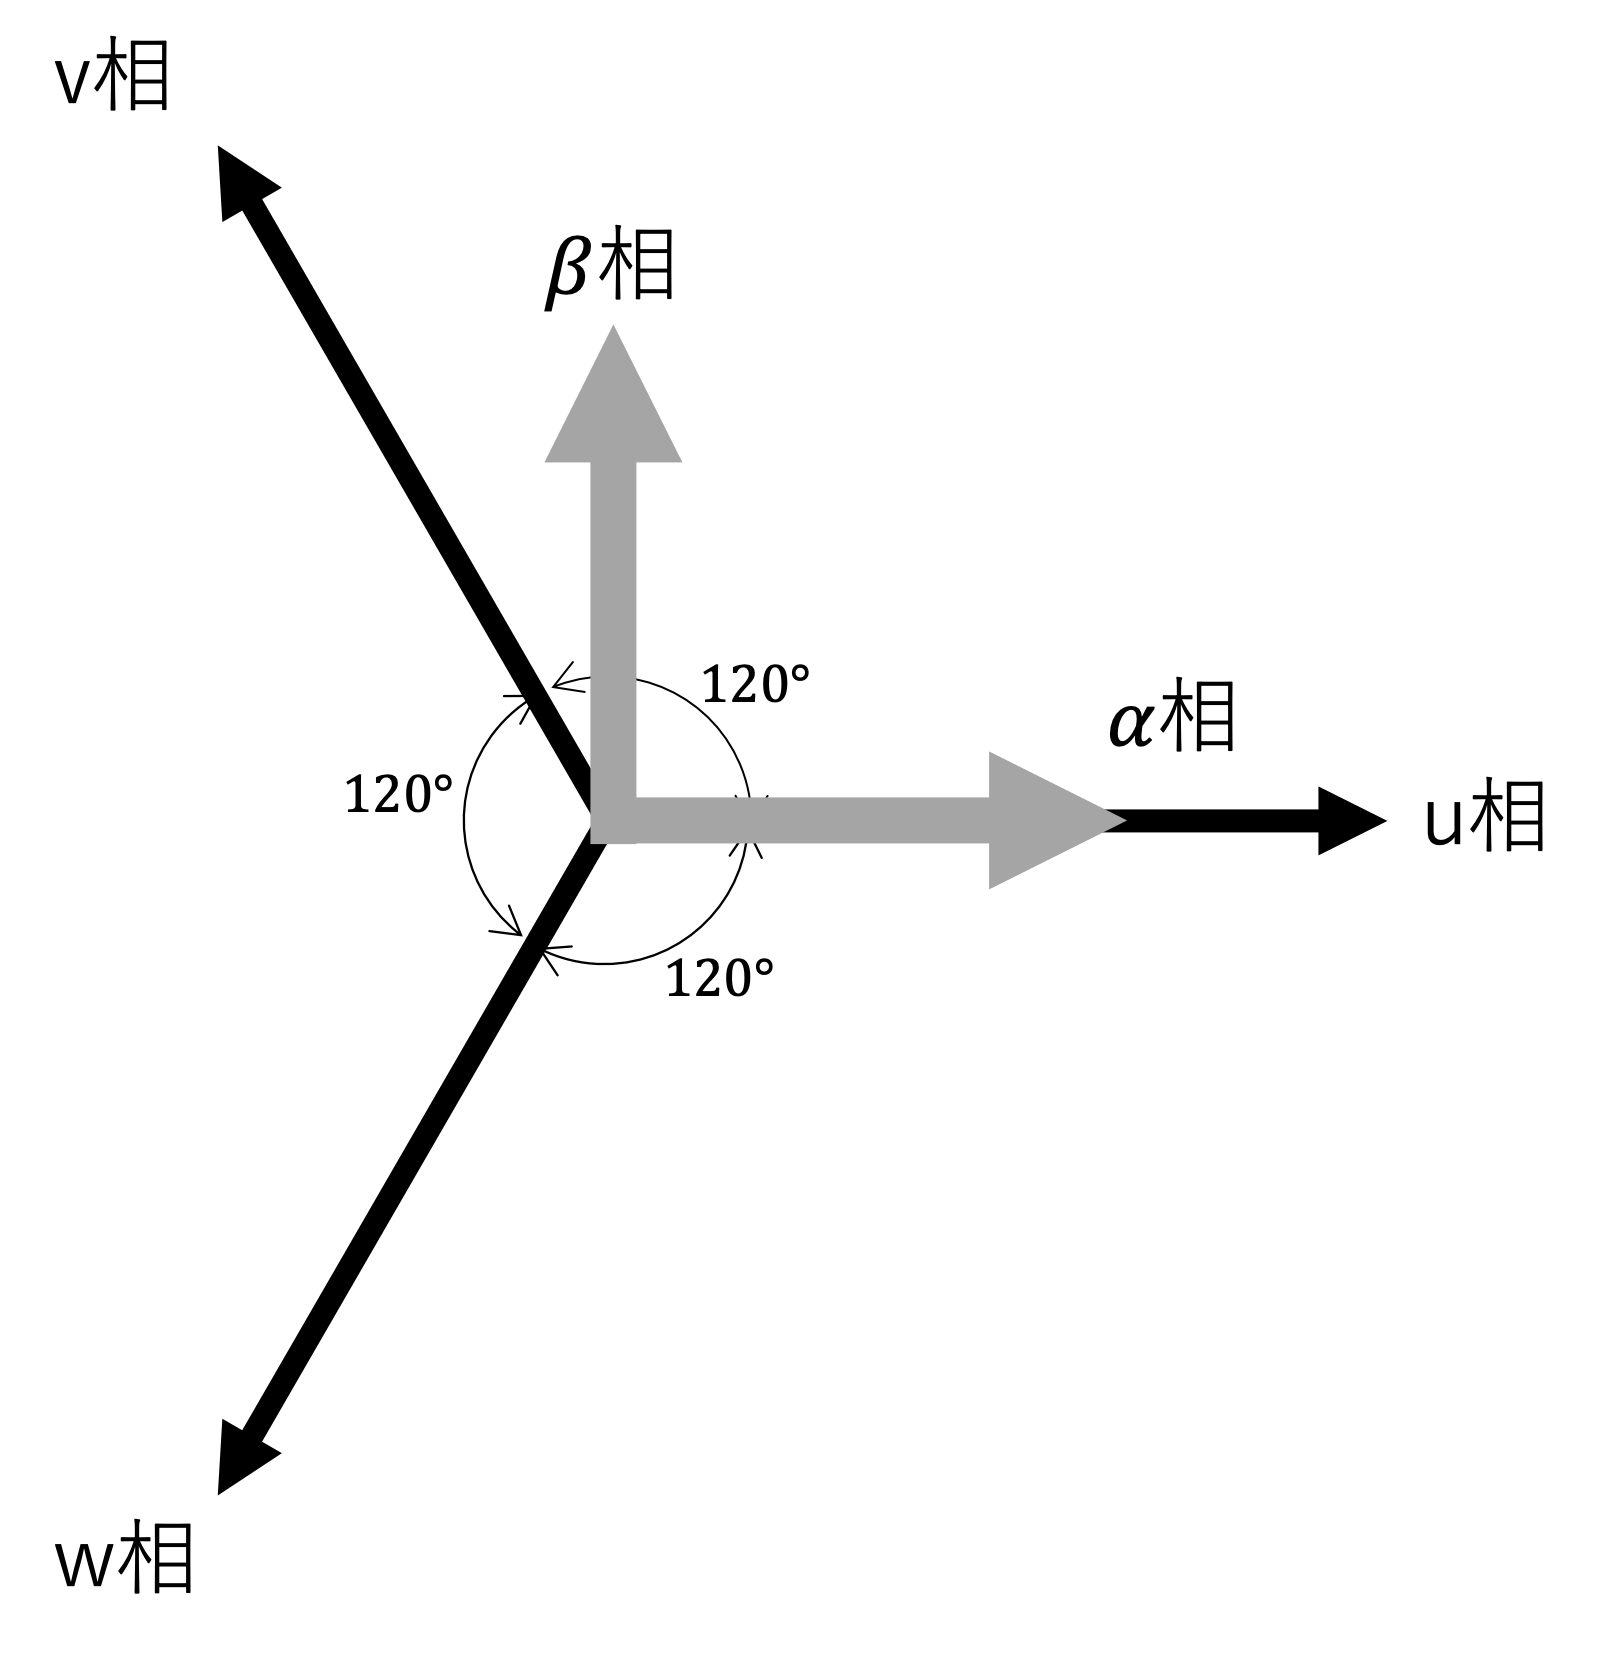
\includegraphics[width=60mm]{image/chapter2/Fig2.2.png}
    \caption{三相交流のベクトルと二相交流のベクトルの関係図}
    \label{Fig2.2}
\end{figure}

図\ref{Fig2.3}に三相二相変換・二相三相変換結果を示す．
三相二相変換とは，三相平衡によって振幅が等しく，隣り合う相の位相が$\frac{2\pi}{3}$だけずれた三相分の交流ベクトルを互いに直交な$\alpha$相と$\beta$相の軸へ成分分解する変換である\cite{3}．これにより三相交流ベクトルは互いに独立した$\alpha$相と$\beta$相のベクトルへ変換される．\par

\begin{figure}[ht]
    \center
    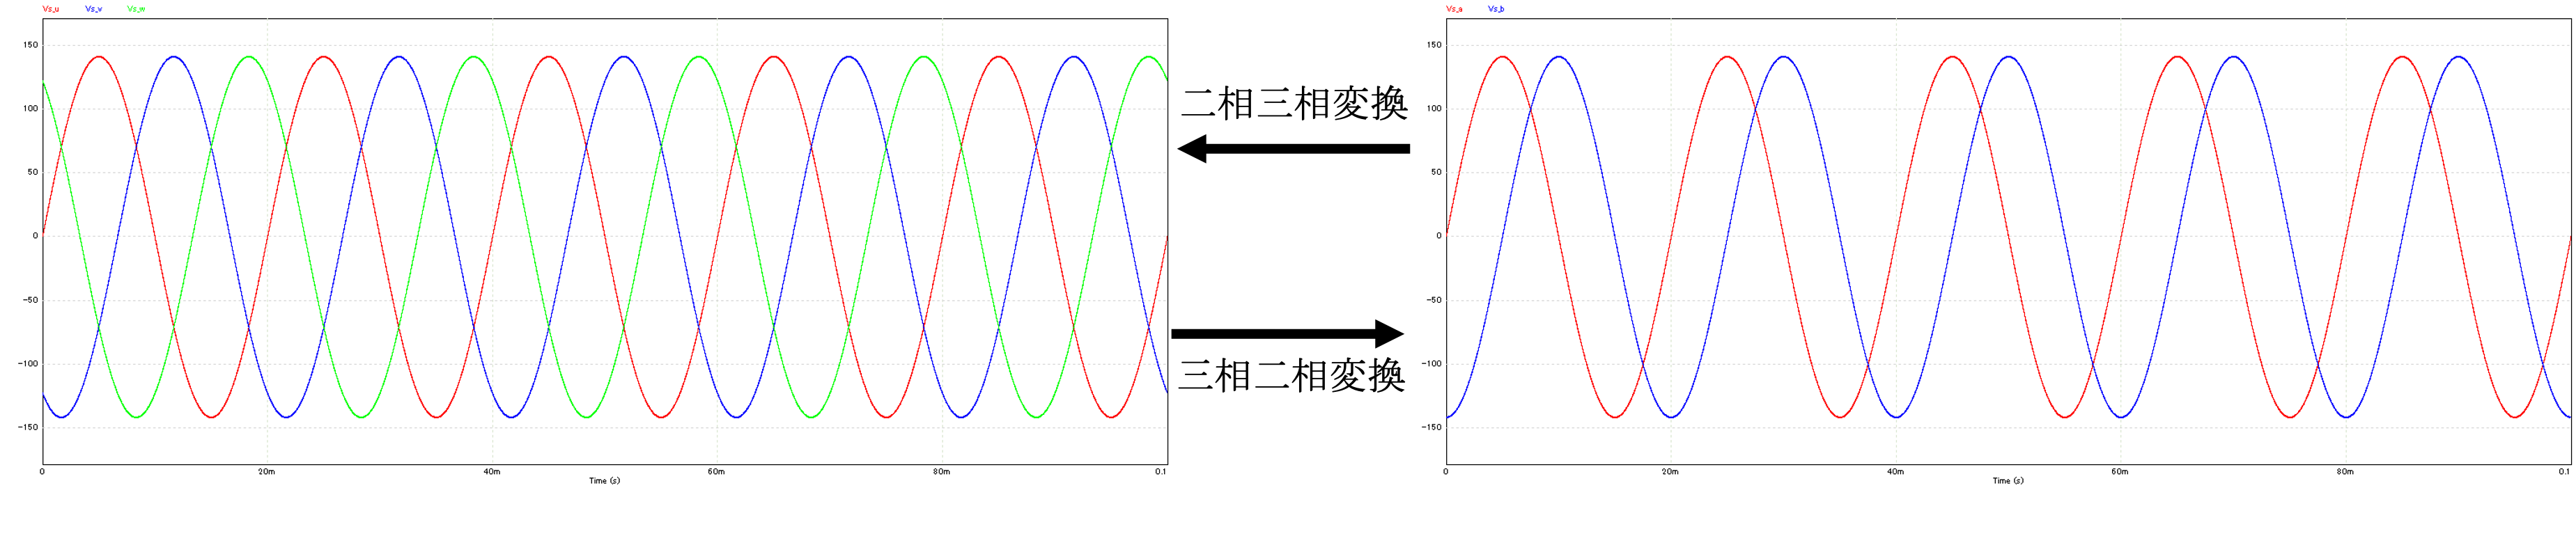
\includegraphics[width=140mm]{image/chapter2/Fig2.3.png}
    \caption{三相二相変換・二相三相変換結果}
    \label{Fig2.3}
\end{figure}

三相二相変換には，相対変換と絶対変換の2種類の方式がある．相対変換では三相と変換後の二相における正弦波の振幅が一致するが，二相における電力量が2/3倍となる．また，絶対変換では，三相と変換後の二相における正弦波の振幅は一致しないが，二相における電力量は一致する．本研究では相対変換を用いる．式(\ref{eq2.1})，(\ref{eq2.2})に三相二相(相間)相対変換，二相三相(相間)相対変換を示す．

\begin{equation}
    \begin{bmatrix}\label{eq2.1}
        x_{\alpha} \\ 
        x_{\beta}       
    \end{bmatrix}
    =\frac{2}{3}
    \begin{bmatrix}
        1 & -\frac{1}{2} & -\frac{1}{2} \\
        0 & -\frac{\sqrt{3}}{2} & -\frac{\sqrt{3}}{2}
    \end{bmatrix}
    \begin{bmatrix}
        x_{u}\\
        x_{v}\\
        x_{w}
    \end{bmatrix}
\end{equation}

\begin{equation}
    \begin{bmatrix} \label{eq2.2}
        x_{u}\\
        x_{v}\\
        x_{w}
    \end{bmatrix}
    =
    \begin{bmatrix}
        1 & 0\\
        -\frac{1}{2} & \frac{\sqrt{3}}{2}\\
        -\frac{1}{2} & -\frac{\sqrt{3}}{2}\\
    \end{bmatrix}
    \begin{bmatrix}
        x_{\alpha} \\
        x_{\beta}
    \end{bmatrix}
\end{equation}

式(\ref{eq2.3})，(\ref{eq2.4})に三相二相(相間)相対変換，二相三相(相間)相対変換を示す．
\begin{equation}
    \begin{bmatrix} \label{eq2.3}
        x_{\alpha} \\
        x_{\beta}
    \end{bmatrix}
    =\sqrt{\frac{2}{3}}
    \begin{bmatrix}
        1 & -\frac{1}{2} & -\frac{1}{2} \\
        0 & -\frac{\sqrt{3}}{2} & -\frac{\sqrt{3}}{2}
    \end{bmatrix}
    \begin{bmatrix}
        x_{u}\\
        x_{v}\\
        x_{w}
    \end{bmatrix}
\end{equation}

\begin{equation}
    \begin{bmatrix} \label{eq2.4}
        x_{u}\\
        x_{v}\\
        x_{w}
    \end{bmatrix}
    =\sqrt{\frac{2}{3}}
    \begin{bmatrix}
        1 & 0\\
        -\frac{1}{2} & \frac{\sqrt{3}}{2}\\
        -\frac{1}{2} & -\frac{\sqrt{3}}{2}\\
    \end{bmatrix}
    \begin{bmatrix}
        x_{\alpha} \\
        x_{\beta}
    \end{bmatrix}
\end{equation}

式(\ref{eq2.5})，(\ref{eq2.6})に三相二相(相間)相対変換，二相三相(相間)相対変換を示す．
\begin{equation}
    \begin{bmatrix} \label{eq2.5}
        x_{\alpha} \\
        x_{\beta}
    \end{bmatrix}
    =\frac{2}{3}
    \begin{bmatrix}
        \frac{1}{2} & 0 & -\frac{1}{2} \\
        0 & \frac{\sqrt{3}}{2} & 0
    \end{bmatrix}
    \begin{bmatrix}
        x_{uv}\\
        x_{vw}\\
        x_{wu}
    \end{bmatrix}
\end{equation}

\begin{equation}
    \begin{bmatrix} \label{eq2.6}
        x_{uv}\\
        x_{vw}\\
        x_{wu}
    \end{bmatrix}
    =\frac{3}{2}
    \begin{bmatrix}
        1  & -\frac{1}{\sqrt{3}}\\
        0  & \frac{2}{\sqrt{3}}\\
        -1 & -\frac{1}{\sqrt{3}}
    \end{bmatrix}
    \begin{bmatrix}
        x_{\alpha} \\
        x_{\beta}
    \end{bmatrix}
\end{equation}

\section{静止座標/回転座標の変換(dq変換)}
図\ref{Fig2.4}に静止座標系・回転座標系の関係図を示す．
静止座標系($\alpha-\beta$軸)上の変数($x_{\alpha}$，$x_{\beta}$)を角度$\theta$で回転する回転座標系($d-q$軸)の変数($x_{d}$，$x_{q}$)に変換する場合やその逆の変換を行うときに用いる制御測である．
\newpage

\begin{figure}[ht]
    \center
    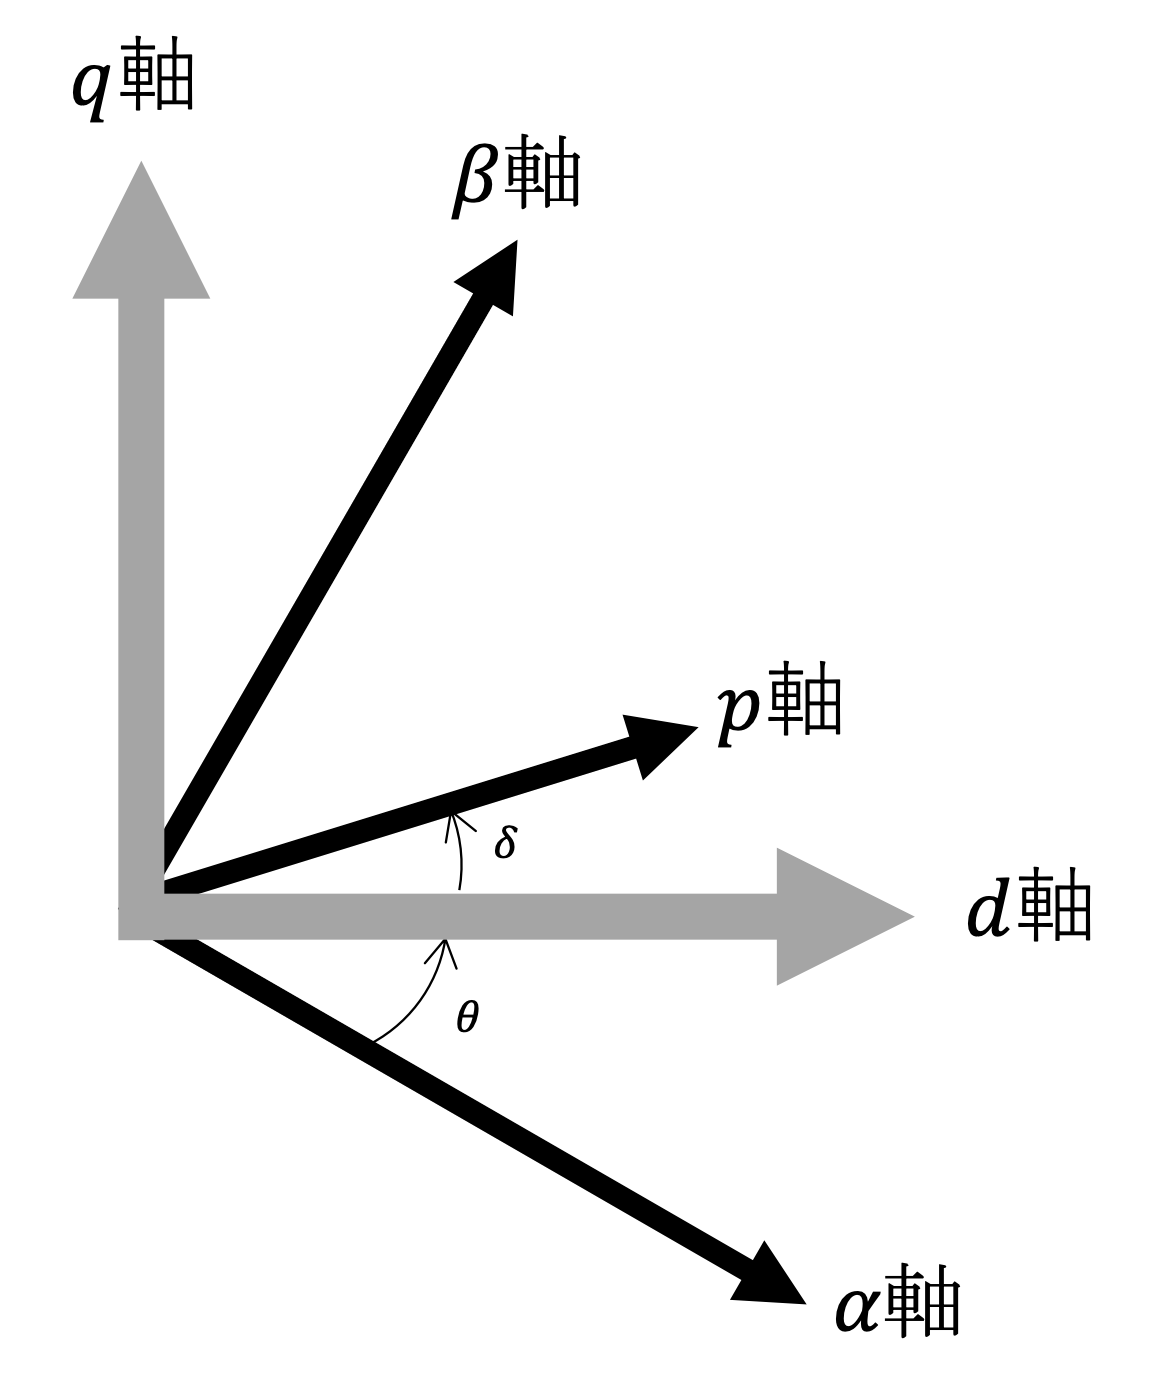
\includegraphics[width=60mm]{image/chapter2/Fig2.4.png}
    \caption{静止座標系・回転座標系の関係図}
    \label{Fig2.4}
\end{figure}

式(\ref{eq2.7})に静止座標系を回転座標系に変換する変換式を示す．
\begin{equation}
    \begin{bmatrix} \label{eq2.7}
        x_{d}\\
        x_{q}
    \end{bmatrix}
    =
    \begin{bmatrix}
        \cos{\theta} & \sin{\theta}\\
        -\sin{\theta}& \cos{\theta}
    \end{bmatrix}
    \begin{bmatrix}
        x_{\alpha} \\
        x_{\beta}
    \end{bmatrix}
\end{equation}

式(\ref{eq2.8})に回転座標系を静止座標系に変換する変換式を示す．
\begin{equation}
    \begin{bmatrix} \label{eq2.8}
        x_{\alpha}\\
        x_{\beta}
    \end{bmatrix}
    =
    \begin{bmatrix}
        \cos{\theta} & -\sin{\theta}\\
        -\sin{\theta}& \cos{\theta}
    \end{bmatrix}
    \begin{bmatrix}
        x_{d} \\
        x_{q}
    \end{bmatrix}
\end{equation}

図\ref{Fig2.5}にdq変換の結果を示す．

\begin{figure}[ht]
    \center
    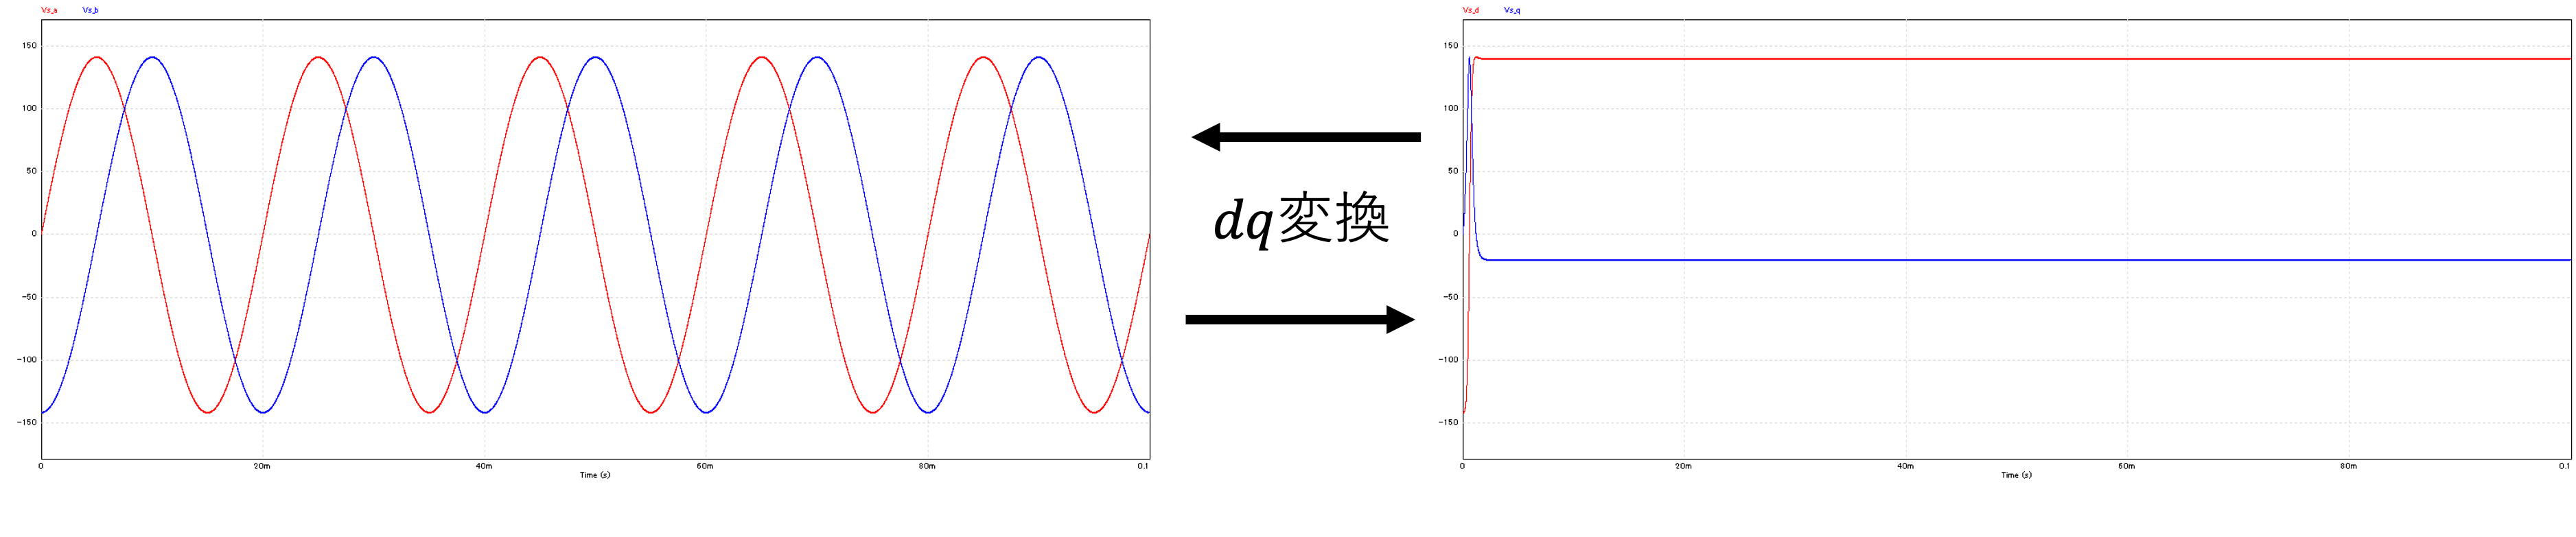
\includegraphics[width=140mm]{image/chapter2/Fig2.5.png}
    \caption{dq変換の結果}
    \label{Fig2.5}
\end{figure}

式(\ref{eq2.7})の様にdq変換を適用し，直交座標系に変換することで振幅相当である$x_{d}$，位相相当である$x_{q}$へ変換することができる．

\section{Phase-Locked-Loop(PLL)}
PLL制御は入力される周期的な信号をもとにフィードバック制御を行い，内部の信号を入力信号の周期に同期する制御である．図\ref{Fig2.6}にPLL制御フロー図を示す．
系統連系システムでは，出力電流を適切に制御するためにインバータの出力電圧の位相と系統電圧の位相を同期させることが必要となり，そのためにPhase-Locked-PLL(PLL)制御を適用する．

\begin{figure}[ht]
    \center
    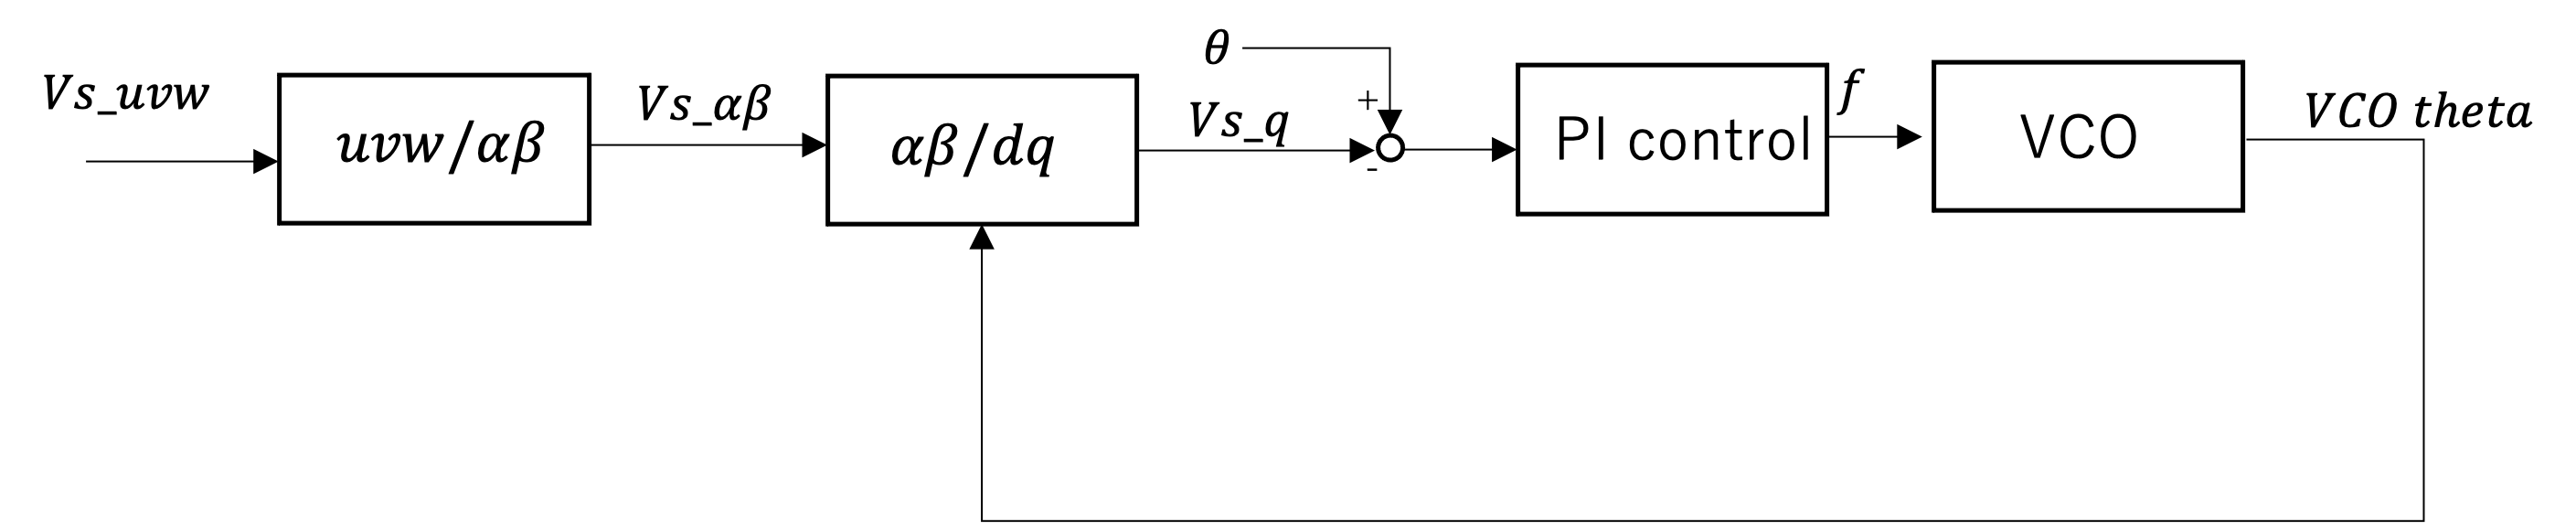
\includegraphics[width=140mm]{image/chapter2/Fig2.6_ver2.png}
    \caption{PLL制御フロー図}
    \label{Fig2.6}
\end{figure}

PLL制御では，系統電圧$V_{s}$に対して三相二相変換を適用することで直交座標系に変換する．その後dq変換を適用することで回転座標系を静止座標系に変換する．dq変換を適用することで振幅相当の$V_{sd}$，位相相当の$V_{sq}$に変換する．検出された位相差$V_{sq}$に対して位相差が0となるようにPI制御を行い，周波数を求める．導出した周波数からコントローラ内部の位相を生成するために，Voltage Controlled Oscillator(VCO)を適用する\cite{3}\cite{4}．


\section{シングルレートデッドビート制御}
デッドビート制御とは制御量を指令値に追従させるためのディジタル制御の一手法である．
図\ref{Fig2.7}に連系リアクトルなし三相系統連系システムの等価回路を示す．

\begin{figure}[ht]
    \center
    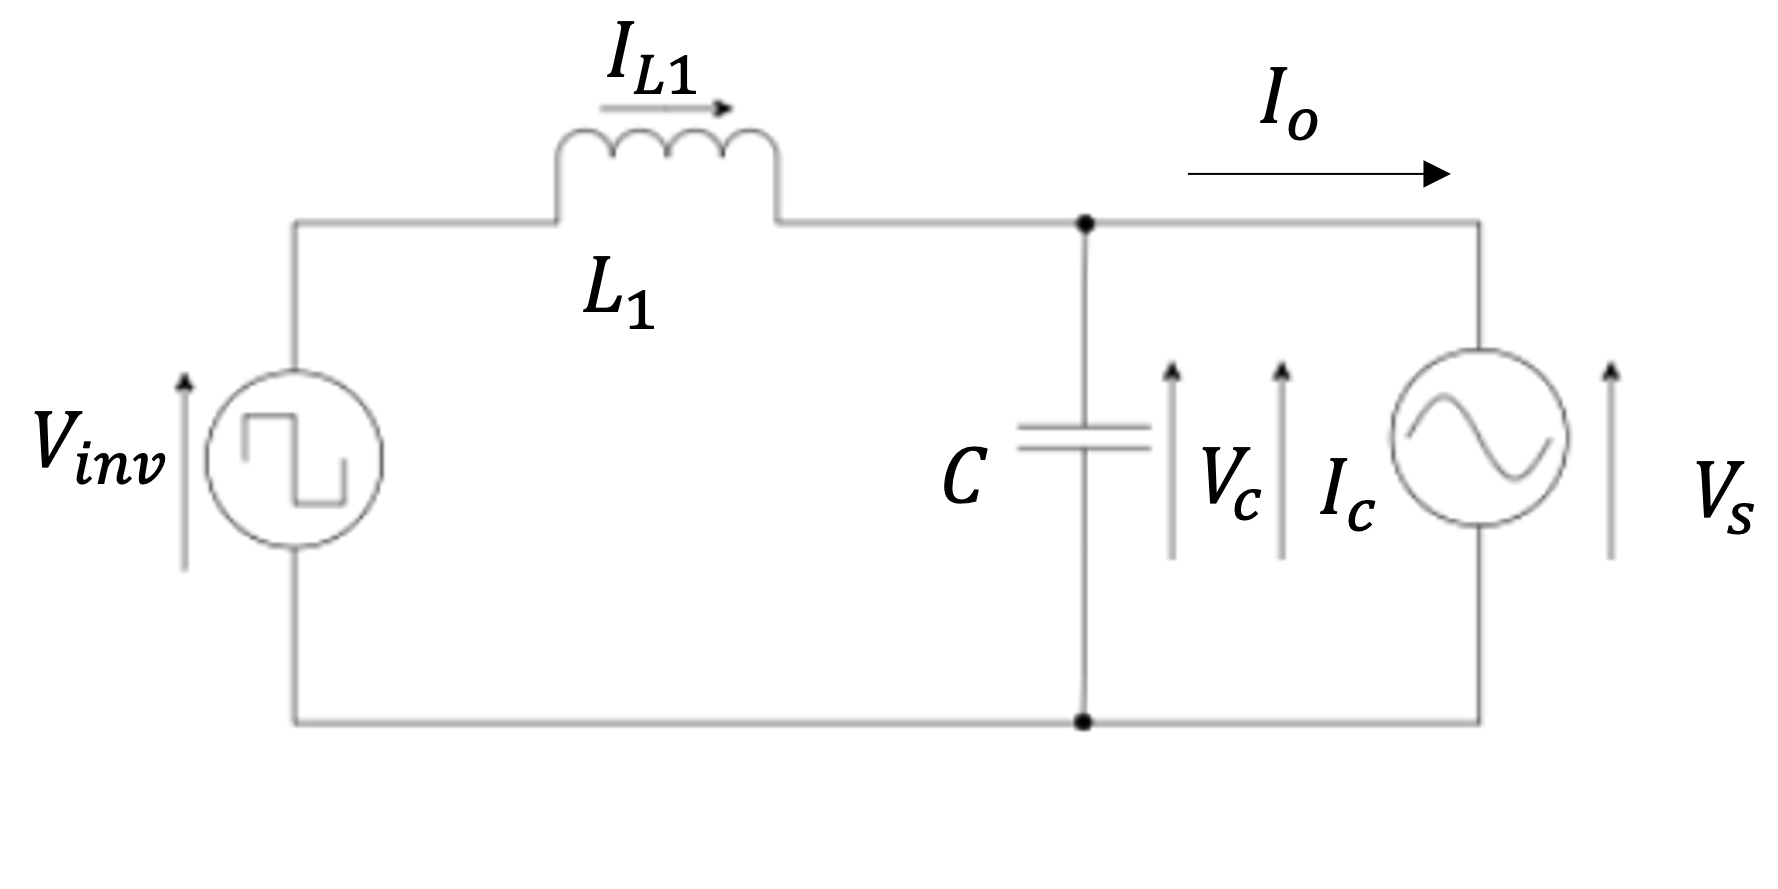
\includegraphics[width=110mm]{image/chapter2/Fig2.7.png}
    \caption{連系リアクトルなし三相系統連系システムの等価回路}
    \label{Fig2.7}
\end{figure}

デッドビート制御は，有限時間内に任意の状態変数を目標値に追従させるための制御であり，サンプリング点において制御量を指令値に追従させることができる．サンプリング点を$KT$，次のサンプリング点を$(K+1)T$としたとき，$(K+1)T$時点における制御量の値を指令値に追従させるために$KT$時点におけるシステムの各状態からインバータの出力電圧パルス指令値$\Delta T(K)$を求め，インバータの出力電圧パルス幅を$\Delta T(K)$とすることで$(K+1)T$時点において制御量を指令値と一致させる．\cite{4}\par
系統連系システムにおける連系インピーダンスの影響を無視した場合のノミナルモデルにおける連続時間状態方程式を示す．

\begin{align}
    &\dot{x}_{\alpha,\beta}=Ax_{\alpha,\beta}+Bu_{\alpha,\beta} \label{eq2.9}\\ &y=cx_{\alpha,\beta}              \label{eq2.10}
\end{align}

ただし式(1)について，

\begin{equation} 
    \begin{split}
       &x_{\alpha,\beta}=
    \begin{bmatrix} 
        I_{L1 \alpha,\beta}  \\
        V_{c\alpha,\beta}   \\
        I_{o\alpha,\beta}     \\
    \end{bmatrix}  \notag  
    ， A=
    \begin{bmatrix}     
        0           & -\frac{1}{L_{1}} &        0             \\
        \frac{1}{C} & 0                &     -\frac{1}{C}     \\ 
        0 & 0 & 0  \\
        0 & 0 & 0   \\
    \end{bmatrix}   \notag  
    &B=
    \begin{bmatrix}     
        \frac{1}{L_{1}}  \\
        0                \\
        0                \\
    \end{bmatrix}   \notag  
    ，u_{\alpha,\beta}=
    \begin{bmatrix}     
        V_{inv}    \\   
    \end{bmatrix}   \notag  
    \end{split}
\end{equation}

である．対象のモデルは連系リアクトル$L_2$を含まないモデルであり，本提案モデルでは，状態量として$I_{L1}$，$V_{c}$，$I_{dis}$，$I_{o}$を使用する．このとき，$I_{L1}$，$V_{c}$，$I_{dis}$の値はシステム上のセンサから取得するが，$I_o$は，センサから取得することができないことを想定しているため，コンデンサ電流$I_c$，インダクタ電流$IL_{1}$，を用いて数値計算を行い導出する．式(\ref{eq2.11})に出力電流の導出式を示す．

\begin{align}
    &I_{o \alpha,\beta}=I_{L1\alpha,\beta}-I_{c\alpha,\beta}   \label{eq2.11}    
\end{align}

式(\ref{eq2.9})の解は式(\ref{eq2.12})で表される．
\begin{align}
    x=e^{At}x(0)+\int_0^t e^{A(t-\tau)} Bu(\tau)d\tau  \label{eq2.12}
\end{align}

ただし，$x_{0}$は初期値である．図\ref{Fig2.8}に出力パルスのモデル図を示す．

\begin{figure}[ht]
    \center
    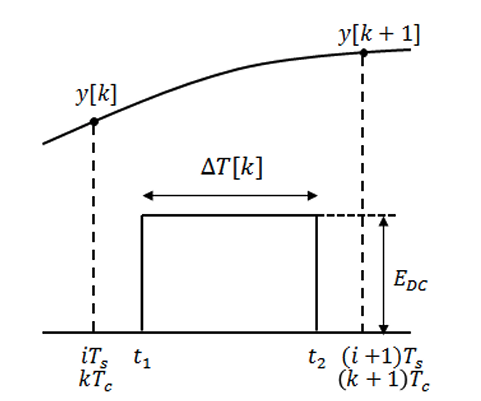
\includegraphics[width=80mm]{image/chapter2/Fig2.8.png}
    \caption{出力パルスのモデル図}
    \label{Fig2.8}
\end{figure}

入力$u$を幅が$\Delta T$のインバータの出力パルスとする．出力パルス$\Delta T$は図\ref{Fig2.8}のように1サンプル区間で左右対称で，大きさは電源電圧$\pm E_{dc}$，系統電圧$V_{s}$は1サンプリング区間において一定値であると仮定する．式(\ref{eq2.12})についてPWMホールドを適用すると，\par
$0\leq t< t_{1}$のときu=0より，式(\ref{eq2.12})は，
 
\begin{align}
    x(t_{1})=e^{A_{v}t}x(0)+\int_{0}^{t_{1}} e^{A(t-\tau)} Bu(\tau)d\tau \label{eq2.13}
\end{align}

$t_{1}\leq t< t_{2}$のときu=$\pm E_{dc}$，より，式(\ref{eq2.11})は，
 
\begin{equation}
    \begin{split}
        x(t_{2})&=e^{A(t_{2}-t_{1})}x(t_{1})+A^{-1}(e^{A(t_{2}-t_{1})}-I_{n})B(\pm E_{dc})+ \int_{t_{1}}^{t_{2}} e^{A(t-\tau)} Bu(\tau)d\tau  \\
        &=e^{A(t_{2}-t_{1})}x(t_{1})+A^{-1}(e^{A(\Delta T)}-I_{n})B(\pm E_{dc})+ \int_{0}^{t_{2}} e^{A(t-\tau)} Bu(\tau)d\tau    \label{eq2.14}
    \end{split}
\end{equation} 

$t_{2}\leq t< T_{s}$のときu=$0$，より，式(\ref{eq2.12})は，

\begin{equation}
    \begin{split}
        x(T_{s})=&e^{A(T_{s}-t_{2})}x(t_{2})+ \int_{t_{2}}^{T_{s}} e^{A(t-\tau)} Bu(\tau)d\tau  \\
        =&e^{A(T_{s}-t_{2})}{e^{A(t_{2})}x(0)+A^{-1}(e^{A(t_{2}-t_{1})}-I_{n})(\pm E_{dc})}\\  
        &+\int_{t_{2}}^{T_{s}} e^{A(t-\tau)} Bu(\tau)d\tau  \\
        =&e^{A(T_{s}}x(0)+e^{A(T_{s}-\Delta T)/2}A^{-1}(e^{A(\Delta T})-I_{n})B(\pm E_{dc})\\
        &+\int_{0}^{T_{s}} e^{A(t-\tau)} Bu(\tau)d\tau  \\ \label{eq2.15}
    \end{split}
\end{equation} 

ただし,
$\Delta T$は図\ref{Fig2.8}から$\Delta T=t_{2}-t_{1}$である．ここで，$e^{A\Delta T/2}$の2次のテイラー級数展開は以下の式で表される．

\begin{align}
    e^{A\Delta T/2} \approx 1+\frac{A\Delta T}{2}+\frac{A^2(\Delta T/2)^2}{2!} \label{eq2.16}
\end{align}

式(\ref{eq2.16})を式(\ref{eq2.15})に代入すると以下の式(\ref{eq2.17})が得られる．

\begin{align}
    x(T_{s})=e^{A(T_{s}}x(0)+e^{AT_{s}/2}A^{-1}B(\pm E_{dc})+\int_{0}^{T_{s}} e^{A(t-\tau)} Bu(\tau)d\tau  \label{eq2.17}
\end{align} 

以上のPWMホールドを用いて式(\ref{eq2.12})を離散化すると離散時間状態方程式は以下の式(\ref{eq2.18})のようになる\cite{5}．

\begin{align}
    x[k+1]=Fx[k]+G\Delta T[k] \label{eq2.18}
\end{align}

式(\ref{eq2.18})について，

\begin{equation} 
    \begin{split}
        F&=e^{ATs}   \\
        &=
    \begin{bmatrix} 
        F_{11} & F_{12} & F_{13}\\
        F_{21} & F_{22} & F_{23}\\
        F_{31} & F_{32} & F_{33}\\
    \end{bmatrix}  \notag  \\
        G&=e^{\frac{ATs}{2}}B(\pm E_{dc})   \\ 
        &=
    \begin{bmatrix}     
        g_{11}  \\
        g_{21}  \\
        g_{31}  \\
    \end{bmatrix}   \notag  \\ 
    \end{split}
\end{equation}

である．　ただし，$F$，$G$の各要素をそれぞれ$F_{ij}$，$G_{ij}$と表現する．$i,j$はそれぞれ第$i$行，第$j$列を意味する．
%各パルス指令信号は式(\ref{eq2.18})の$\Delata T[k]$について解くことで導出することができる．$\alpha $相，$\beta $相，の各パルス指令信号$\Delta T_{\alpha } [k]$，$\Delta T_{\beta }[k]$は，式(\ref{eq2.19})，(\ref{eq2.20})のように表すことができる．

\begin{equation}
    \begin{split}
        \Delta T_{\alpha [k]}=&\frac{I_{L\alpha}[k+1]-z11 I_{L1\alpha}[k]-z12 V_{c\alpha}[k]-z_{13} I_{o\alpha}[k]}{g11}  \label{eq2.19}
    \end{split}
\end{equation}

\begin{equation}
    \begin{split}
        \Delta T_{\beta [k]}=&\frac{I_{L\beta}[k+1]-z11 I_{L1\beta}[k]-z12 V_{c\beta}[k]-z_{13} I_{o\beta}[k]}{g11}    \label{eq2.20}
    \end{split}
\end{equation}

式(\ref{eq2.19})，(\ref{eq2.20})の様に導出された$\alpha$相と$\beta$相の操作量に対して二相三相変換することでU相，V相，W相の操作量を生成する．その後，導出した各相の操作量と三角波を比較するPWM制御を適用することでインバータのゲート信号を生成する．

\section{外乱補償型シングルレートデッドビート制御}
図\ref{Fig2.9}に外乱成分を追加した連系リアクトルなし三相系統連系システムの等価回路を示す．外乱補償型シングルレートデッドビート制御とは，シングルレートデッドビート制御に外乱成分を補償するための項を追加した制御である．先行研究では，外乱補償型シングルレートデッドビート制御を用いることでパラメータ変動等によって制御対象が案ノミナルとなった場合に外乱成分を抑制することでシステムのロバスト性が向上することが判明している\cite{7}．

\newpage
\begin{figure}[ht]
    \center
    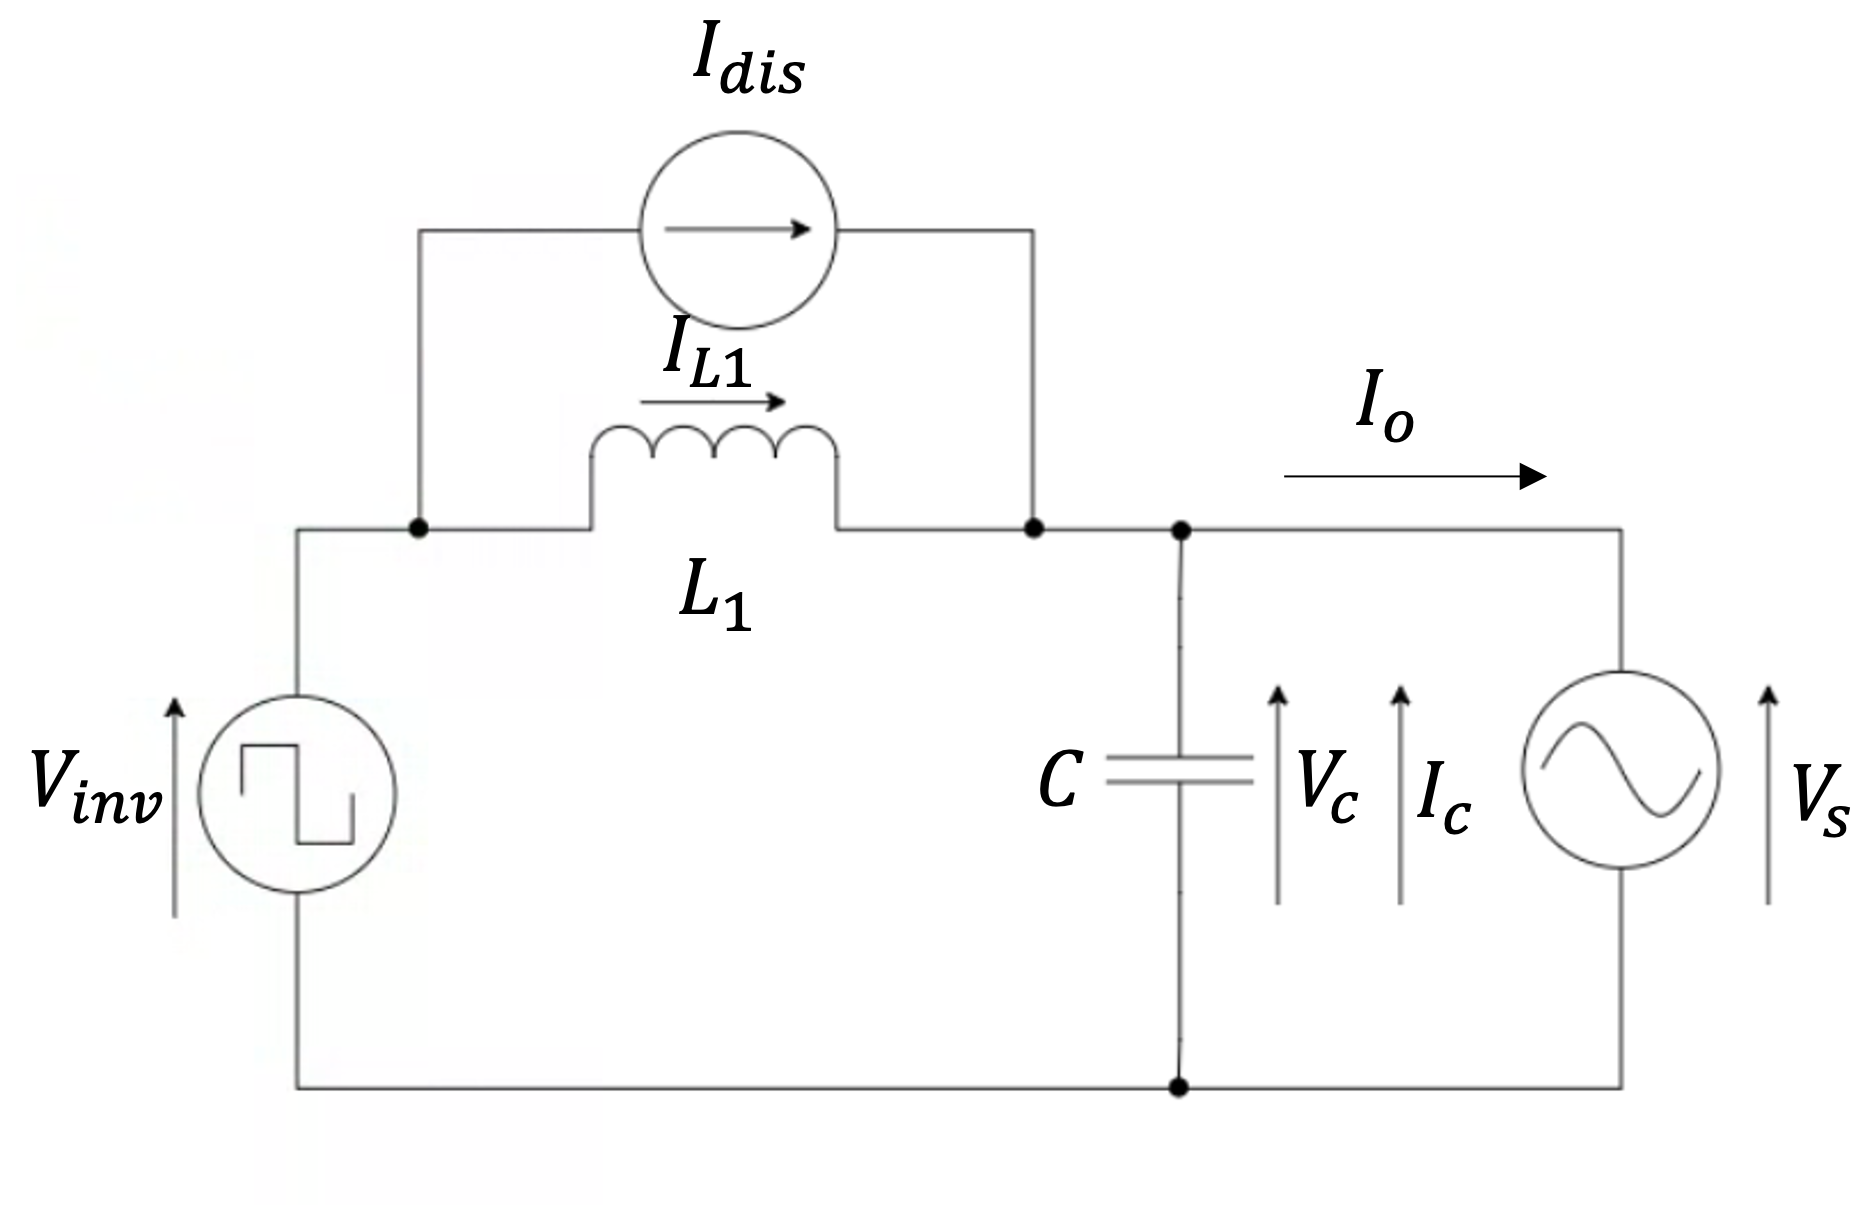
\includegraphics[width=80mm]{image/chapter2/Fig2.9.png}
    \caption{外乱成分を追加した連系リアクトルなし三相系統連系システムの等価回路}
    \label{Fig2.9}
\end{figure}

本研究において，外乱として想定するものは外乱電流であり，ノミナル時における出力電流以外を外乱電流とする．

\begin{align}
    &\dot{x}_{\alpha,\beta}=Ax_{\alpha,\beta}+Bu_{\alpha,\beta} \label{eq2.21}\\ &y=cx_{\alpha,\beta}              \label{eq2.22}
\end{align}

ただし式(\ref{eq2.21})について，

\begin{equation} 
    \begin{split}
       &x_{\alpha,\beta}=
    \begin{bmatrix} 
        I_{L1 \alpha,\beta}  \\
        V_{c\alpha,\beta}   \\
        I_{o\alpha,\beta}     \\
        I_{dis\alpha,\beta} \\
    \end{bmatrix}  \notag  
    ， A=
    \begin{bmatrix}     
        0           & -\frac{1}{L_{1}} &        0           & 0  \\
        \frac{1}{C} & 0                &     -\frac{1}{C}     &  \frac{1}{C} \\ 
        0 & 0 & 0 & 0  \\
        0 & 0 & 0 & 0  \\
    \end{bmatrix}   \notag  
    &B=
    \begin{bmatrix}     
        \frac{1}{L_{1}}  \\
        0                \\
        0                \\
        0                \\
    \end{bmatrix}   \notag  
    ，u_{\alpha,\beta}=
    \begin{bmatrix}     
        V_{inv}    \\   
    \end{bmatrix}   \notag  
    \end{split}
\end{equation}

である．対象のモデルは連系リアクトル$L_2$を含まないモデルであり，本モデルでは，状態量として$I_{L1}$，$V_{c}$，$I_{dis}$，$I_{o}$を使用する．このとき，$I_{L1}$，$V_{c}$，$I_{dis}$の値はシステム上のセンサから取得するが，$I_o$は，センサから取得することができないことを想定しているため，にコンデンサ電流$I_c$，インダクタ電流$IL_{1}$，外乱電流$I_{dis}$を用いて数値計算を行い導出する．式(\ref{eq2.23})に出力電流の導出式を示す．

\begin{align}
    &I_{o \alpha,\beta}=I_{L1\alpha,\beta}+I_{dis\alpha,\beta}-I_{c\alpha,\beta}   \label{eq2.23}    
\end{align}

式(\ref{eq2.21})の解は式(\ref{eq2.24})で表される．
\begin{align}
    x=e^{At}x(0)+\int_0^t e^{A(t-\tau)} Bu(\tau)d\tau  \label{eq2.24}
\end{align}

ただし，$x_{0}$は初期値である．入力$u$を幅が$\Delta T$のインバータの出力パルスとする．出力パルス$\Delta T$は図\ref{Fig2.8}のように1サンプル区間で左右対称で，大きさは電源電圧$\pm E_{dc}$，系統電圧$V_{s}$は1サンプリング区間において一定値であると仮定する．式(\ref{eq2.24})についてPWMホールドを適用すると\par
$0\leq t< t_{1}$のときu=0より，式(\ref{eq2.24})は，
 
\begin{align}
    x(t_{1})=e^{A_{v}t}x(0)+\int_{0}^{t_{1}} e^{A(t-\tau)} BV_{s}(\tau)d\tau \label{eq2.25}
\end{align}

$t_{1}\leq t< t_{2}$のときu=$\pm E_{dc}$，より，式(\ref{eq2.24})は，
 
\begin{equation}
    \begin{split}
        x(t_{2})&=e^{A(t_{2}-t_{1})}x(t_{1})+A^{-1}(e^{A(t_{2}-t_{1})}-I_{n})B(\pm E_{dc})+ \int_{t_{1}}^{t_{2}} e^{A(t-\tau)} BV_{s}(\tau)d\tau  \\
        &=e^{A(t_{2}-t_{1})}x(t_{1})+A^{-1}(e^{A(\Delta T)}-I_{n})B(\pm E_{dc})+ \int_{0}^{t_{2}} e^{A(t-\tau)} BV_{s}(\tau)d\tau    \label{eq2.26}
    \end{split}
\end{equation} 

$t_{2}\leq t< T_{s}$のときu=$0$，より，式(\ref{eq2.24})は，

\begin{equation}
    \begin{split}
        x(T_{s})=&e^{A(T_{s}-t_{2})}x(t_{2})+ \int_{t_{2}}^{T_{s}} e^{A(t-\tau)} BV_{s}(\tau)d\tau  \\
        =&e^{A(T_{s}-t_{2})}{e^{A(t_{2})}x(0)+A^{-1}(e^{A(t_{2}-t_{1})}-I_{n})(\pm E_{dc})}\\  
        &+\int_{t_{2}}^{T_{s}} e^{A(t-\tau)} BV_{s}(\tau)d\tau  \\
        =&e^{A(T_{s}}x(0)+e^{A(T_{s}-\Delta T)/2}A^{-1}(e^{A(\Delta T})-I_{n})B(\pm E_{dc})\\
        &+\int_{0}^{T_{s}} e^{A(t-\tau)} BV_{s}(\tau)d\tau  \\ \label{eq2.27}
    \end{split}
\end{equation} 

式(\ref{eq2.17})を式(\ref{eq2.27})に代入すると以下の式(\ref{eq2.28})が得られる．

\begin{align}
    x(T_{s})=e^{A(T_{s}}x(0)+e^{AT_{s}/2}A^{-1}B(\pm E_{dc})+\int_{0}^{T_{s}} e^{A(t-\tau)} BV_{s}(\tau)d\tau   \label{eq2.28}
\end{align} 

以上のPWMホールドを用いて式(\ref{eq2.24})を離散化すると離散時間状態方程式は以下の式のようになる．

\begin{align}
    x[k+1]=Fx[k]+G\Delta T[k] \label{eq2.29}
\end{align}

式(\ref{eq2.29})について，

\begin{equation} 
    \begin{split}
        F&=e^{ATs}   \\
        &=
    \begin{bmatrix} 
        F_{11} & F_{12} & F_{13} & F_{14}\\
        F_{21} & F_{22} & F_{23} & F_{24}\\
        F_{31} & F_{32} & F_{33} & F_{34}\\
        F_{41} & F_{42} & F_{43} & F_{44}\\
    \end{bmatrix}  \notag  \\
        G&=e^{\frac{ATs}{2}}B(\pm E_{dc})   \\ 
        &=
    \begin{bmatrix}     
        g_{11}  \\
        g_{21}  \\
        g_{31}  \\
        g_{41}  \\
    \end{bmatrix}   \notag  \\ 
    \end{split}
\end{equation}

である．　ただし，$F$，$G$の各要素をそれぞれ$F_{ij}$，$G_{ij}$と表現する．$i,j$はそれぞれ第$i$行，第$j$列を意味する．
%各パルス指令信号は式(\ref{eq2.29})の$\Delata T[k]$について解くことで導出することができる．$\alpha $相，$\beta $相，の各パルス指令信号$\Delta T_{\alpha } [k]$，$\Delta T_{\beta }[k]$は，式(\ref{eq2.30})，(\ref{eq2.31})のように表すことができる．

\begin{equation}
    \begin{split}
        \Delta T_{\alpha [k]}=&\frac{I_{L\alpha}[k+1]-z11 I_{L1\alpha}[k]-z12 V_{c\alpha}[k]-z_{13} I_{o\alpha}[k]-z14 I_{dis\alpha}[k]}{g11}  \label{eq2.30}
    \end{split}
\end{equation}

\begin{equation}
    \begin{split}
        \Delta T_{\beta [k]}=&\frac{I_{L\beta}[k+1]-z11 I_{L1\beta}[k]-z12 V_{c\beta}[k]-z_{13} I_{o\beta}[k]-z14 I_{dis\beta}[k]}{g11}    \label{eq2.31}
    \end{split}
\end{equation}

式(\ref{eq2.30})，(\ref{eq2.31})の様に導出された$\alpha$相と$\beta$相の操作量に対して二相三相変換することでU相，V相，W相の操作量を生成する．その後，導出した各相の操作量と三角波を比較するPWM制御を適用することでインバータのゲート信号を生成する．

\section{インダクタ電流指令値生成}
本研究においてデッドビート制御における制御量はフィルタインダクタ$L_{1}$に流れる電流$I_{L1}$である．制御対象であるインダクタ電流の指令値$I_{L1 ref}$はノミナル電流の振幅$I_{nom amp}$，PLL制御によって導出した位相角VCOを用いて以下の式(\ref{eq2.32})で表される．
\begin{align}
    I_{L1 ref}=I_{nom amp}\times \sin(VCO) \label{eq2.32}
\end{align}

式(\ref{eq2.32})では，PLL制御によって導出された系統電圧のU相の位相に同期した位相角を元に指令値の生成を行なっている．

\section{マルチサンプリングデッドビート制御}
図\ref{Fig2.10}にマルチサンプリング制御のイメージ図を示す．

\newpage

\begin{figure}[ht]
    \center
    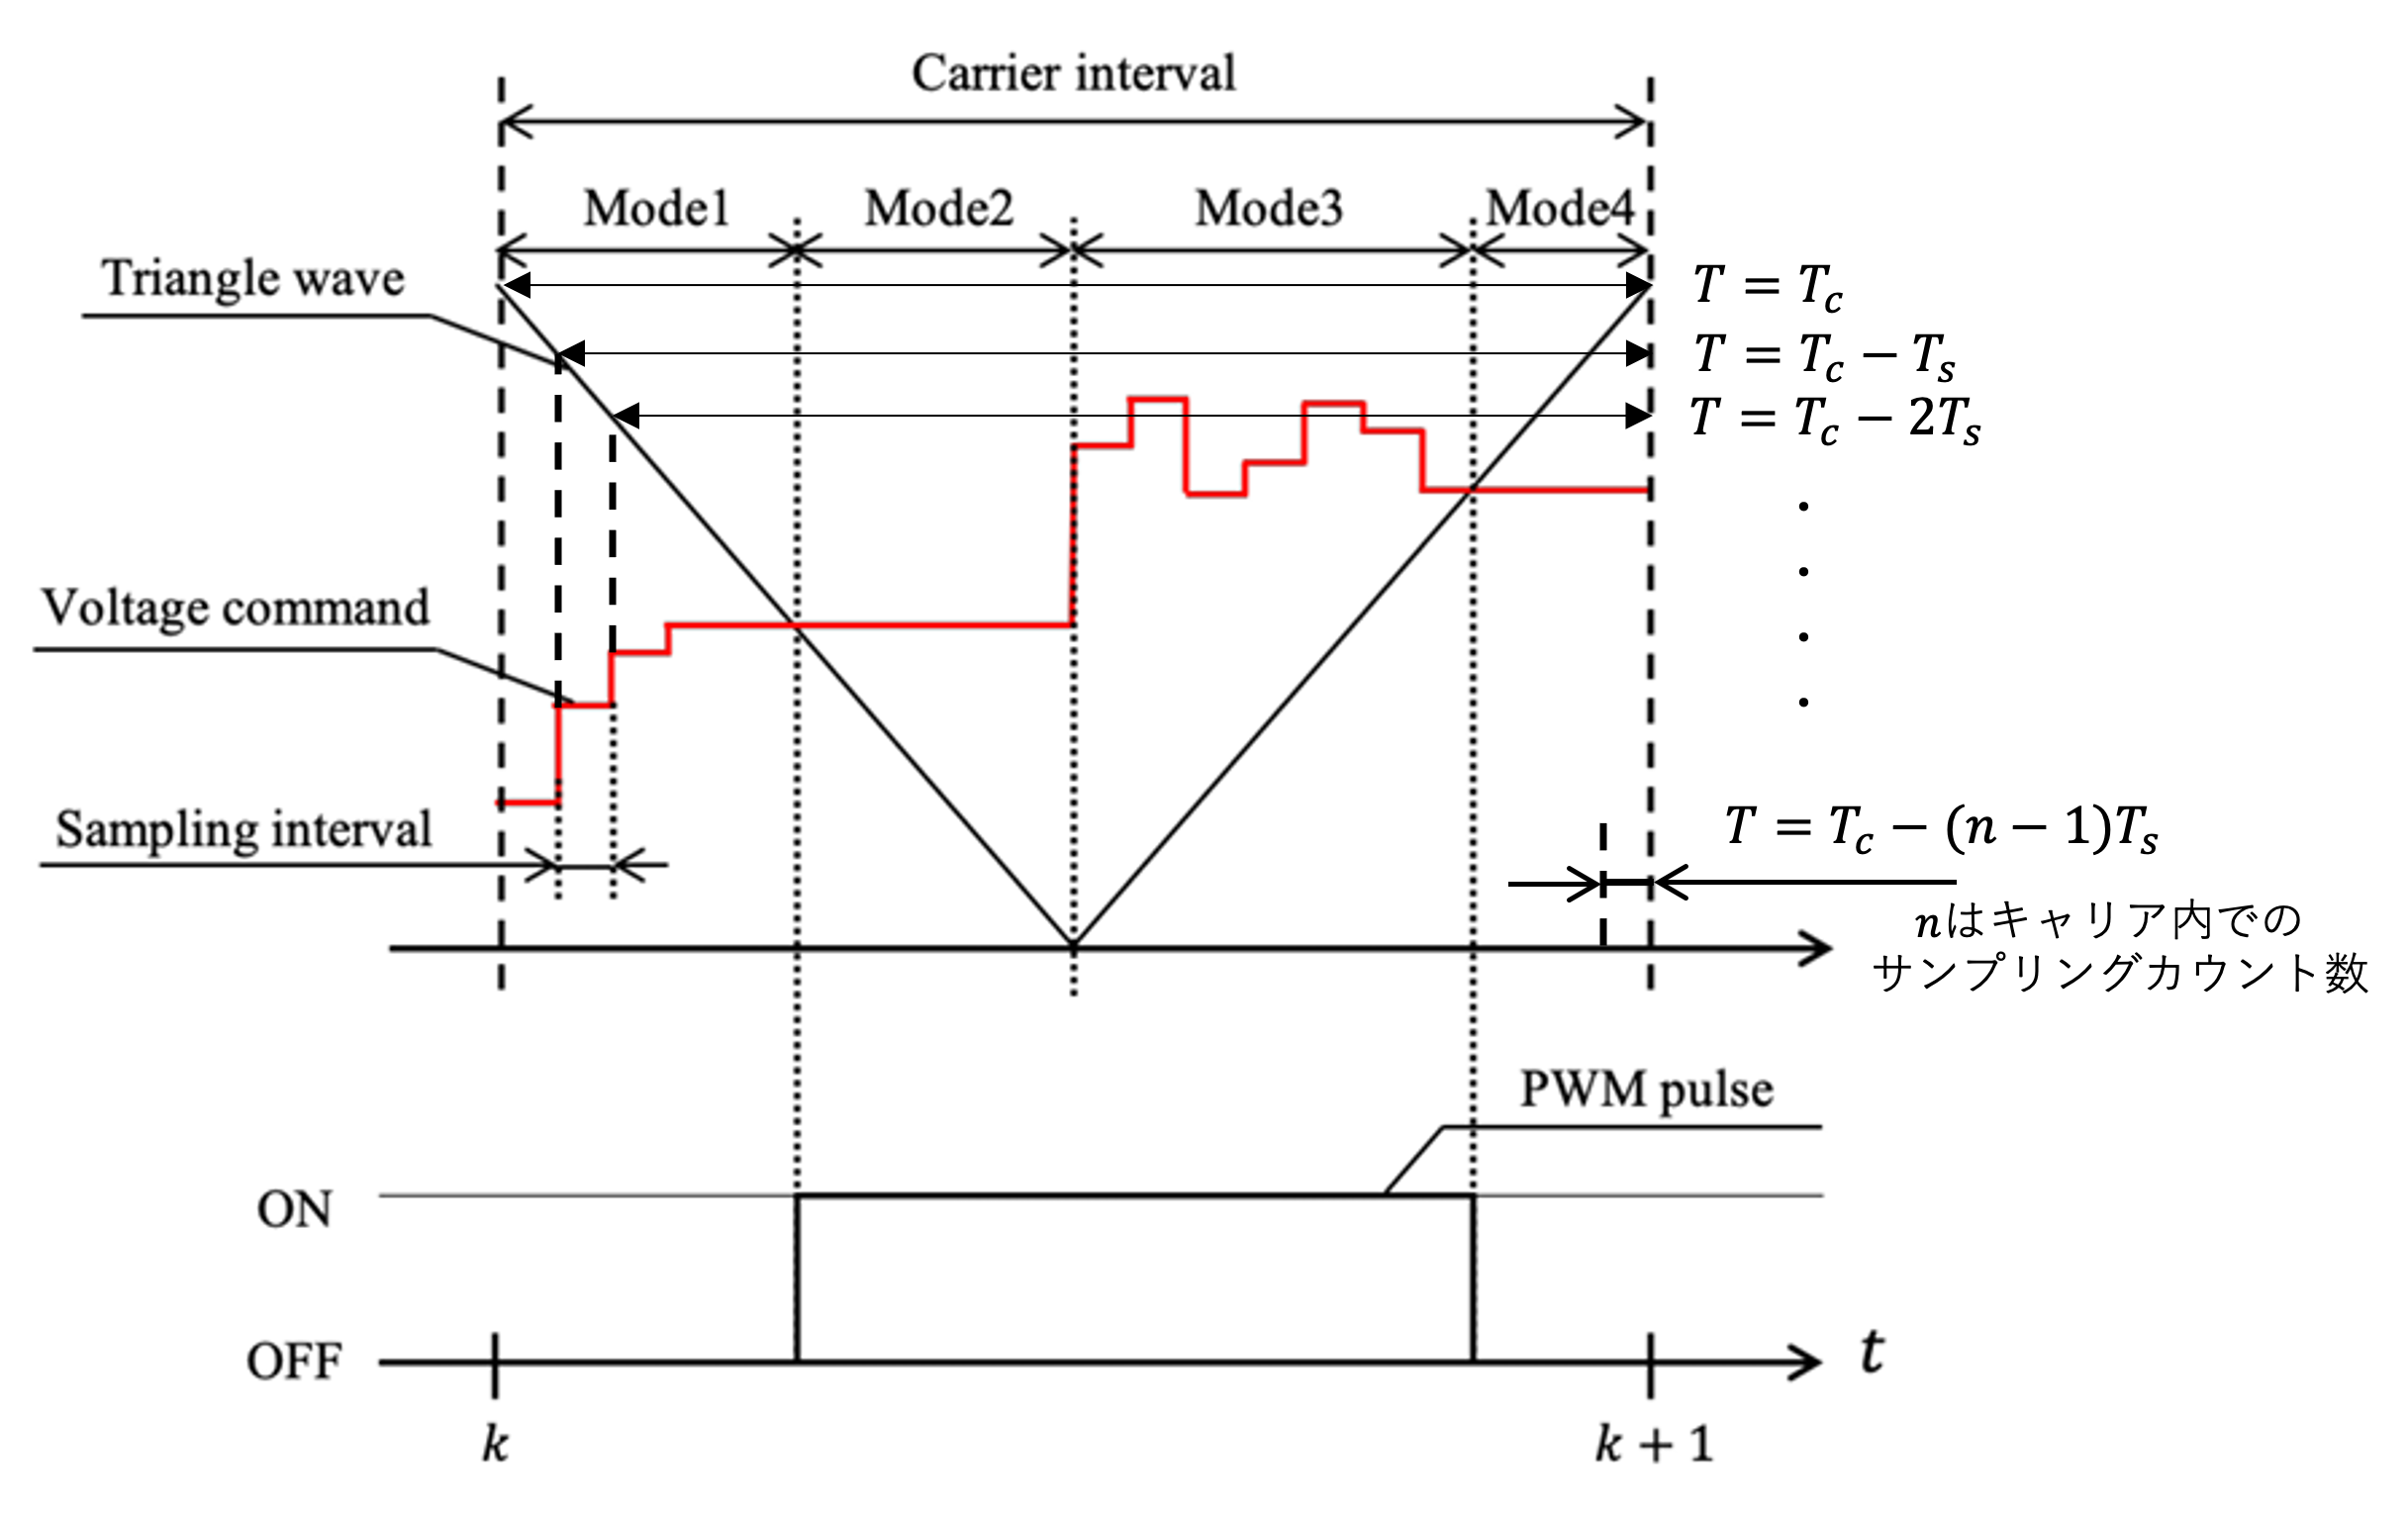
\includegraphics[width=110mm]{image/chapter2/Fig2.10.png}
    \caption{マルチサンプリング制御のイメージ図}
    \label{Fig2.10}
\end{figure}

マルチサンプリングデッドビート制御とは，キャリア周期$T_{c}$に対してでサンプリング周期$T_{s}$を小さくすることでとパルス指令の演算を複数回行うマルチサンプリング手法をデッドビート制御に適用したものである\cite{8}．\par
マルチサンプリングデッドビート制御では，PWMパルスの二度切りを防止するために動作モードが４つに分かれている．それぞれをmode1，mode2,mode3,mode4としている．以下に各モードの説明を示す．\\
\\
mode1：パルスのONタイミングを決定するmodeであり，1サンプリング毎にパルス指令値の演算を行い，三角波と等しくなった点をON時間とする．\\
\\
mode2：パルスがOFFになることを防ぐためのmodeであり，mode1の三角波とパルス指令値が等しくなった点からキャリア周期の半分までmode1の出力を保持する．\\
\\
mode3:パルスのOFFタイミングを決定するmodeであり，1サンプリング毎にパルス指令値の演算を行い，三角波と等しくなった点をOFF時間とする．\\
\\
mode4：パルスがONになることを防ぐためのmodeであり，mode3の三角波とパルス指令値が等しくなった点から次の周期の開始までmode3の出力を保持する．\\